\documentclass[portrait]{seminar}
%\usepackage{pandora}
\usepackage{color}
\usepackage{fancybox}
\usepackage{alltt}
\usepackage{epsfig}
\usepackage{rail}
\usepackage{bar}
\usepackage{url}
\usepackage{rotating}
\usepackage[normalem]{ulem}
\usepackage{latexsym}
\usepackage{amsmath}

\begin{document}

\boldmath
\newcommand{\RA}{$\rightarrow$}
\newcommand{\LL}{\mbox{$[$\hspace{-0.15em}$[$}}
\newcommand{\RR}{\mbox{$]$\hspace{-0.15em}$]$}}
\newcommand{\CC}[1]{\mbox{\tt $\LL$#1$\RR$}}

\slideframe{shadow}

%%% Activate one of these to get either Aarhus style or McGill style 
%%% by putting a #1 in the appropriate line.
\newcommand{\mcgill}[1]{#1}
\newcommand{\aarhus}[1]{}

%%% Define this to be the name of your term
\newcommand{\courseterm}{Fall 2012}




\aarhus{
\newpagestyle{dOvsstyle}{dOvs'98 Week 39 \hfil Abstract syntax trees}{\hfil \thepage}
}

\mcgill{
\newpagestyle{dOvsstyle}{COMP 520 \courseterm  \hfil Abstract syntax trees (\thepage)}{}
}
\slidepagestyle{dOvsstyle}

\begin{slide*}
\begin{tabbing}
\aarhus{{\Large\bf Week 39}\\}
~\\
{\Huge\bf Abstract}\\ ~\\ {\Huge\bf syntax trees}\\
\end{tabbing}

\begin{center}
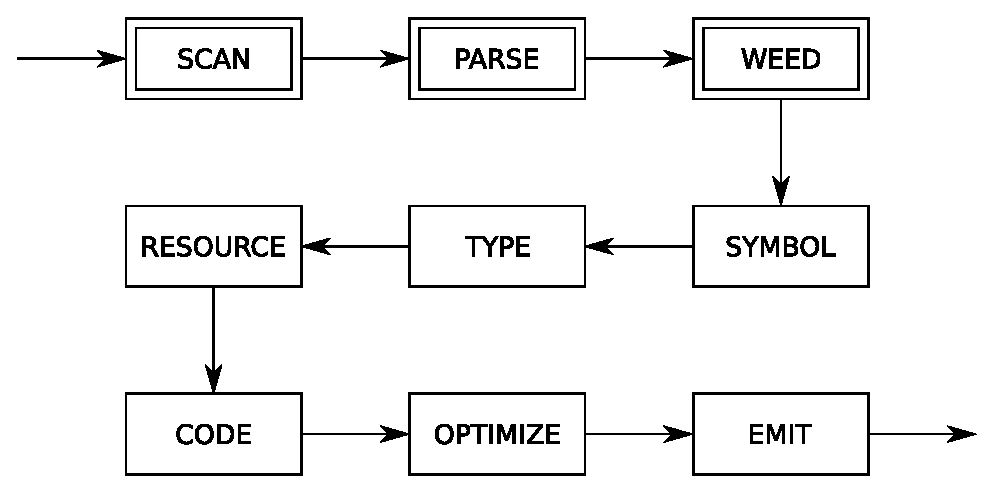
\psfig{file=figs/scan_parse_weed.eps,width=20em}
\end{center}

\vfil
\end{slide*}

\begin{slide*}
A compiler {\em pass} is a traversal of the program.
A compiler {\em phase} is a group of related passes.

A {\em one-pass} compiler scans the program only once.  It is
naturally single-phase.  The following all happen at the same time:

\begin{itemize}
\item scanning
\item parsing
\item weeding
\item symbol table creation
\item type checking
\item resource allocation
\item code generation
\item optimization
\item emitting
\end{itemize}
\vfil
\end{slide*}

\begin{slide*}
This is a terrible methodology:
\begin{itemize}
\item it ignores natural modularity;
\item it gives unnatural scope rules; and
\item it limits optimizations.
\end{itemize}

However, it used to be popular:
\begin{itemize}
\item it's fast (if your machine is slow); and
\item it's space efficient (if you only have 4K).
\end{itemize}

A modern {\em multi-pass} compiler uses 5--15 phases, some of which
may have many individual passes: you should skim through the
optimization section of `man gcc' some time!
\vfil
\end{slide*}
 
\begin{slide*}
A multi-pass compiler needs an {\em intermediate representation} of
the program between passes.

We could use a parse tree, or {\em concrete syntax tree} (CST):

\begin{center}
\setlength{\unitlength}{0.00041500in}%
%
\begingroup\makeatletter\ifx\SetFigFont\undefined%
\gdef\SetFigFont#1#2#3#4#5{%
  \reset@font\fontsize{#1}{#2pt}%
  \fontfamily{#3}\fontseries{#4}\fontshape{#5}%
  \selectfont}%
\fi\endgroup%
\begin{picture}(2787,3735)(3226,-5113)
\thicklines
\put(4201,-1561){\line(-3,-2){900}}
\put(4201,-1561){\line( 0,-1){600}}
\put(4201,-1561){\line( 3,-2){900}}
\put(3301,-2461){\line( 0,-1){600}}
\put(3301,-3361){\line( 0,-1){600}}
\put(3301,-4261){\line( 0,-1){600}}
\put(5101,-2461){\line(-3,-2){900}}
\put(5101,-2461){\line( 0,-1){600}}
\put(5101,-2461){\line( 3,-2){900}}
\put(4201,-3361){\line( 0,-1){600}}
\put(4201,-4261){\line( 0,-1){600}}
\put(6001,-3361){\line( 0,-1){600}}
\put(4126,-1486){\makebox(0,0)[lb]{\smash{\SetFigFont{8}{14.4}{\familydefault}{\mddefault}{\updefault}$E$}}}
\put(3226,-2386){\makebox(0,0)[lb]{\smash{\SetFigFont{8}{14.4}{\familydefault}{\mddefault}{\updefault}$E$}}}
\put(4100,-2386){\makebox(0,0)[lb]{\smash{\SetFigFont{8}{14.4}{\familydefault}{\mddefault}{\updefault}+}}}
\put(5026,-2386){\makebox(0,0)[lb]{\smash{\SetFigFont{8}{14.4}{\familydefault}{\mddefault}{\updefault}$T$}}}
\put(3226,-3286){\makebox(0,0)[lb]{\smash{\SetFigFont{8}{14.4}{\familydefault}{\mddefault}{\updefault}$T$}}}
\put(3226,-4186){\makebox(0,0)[lb]{\smash{\SetFigFont{8}{14.4}{\familydefault}{\mddefault}{\updefault}$F$}}}
\put(3226,-5086){\makebox(0,0)[lb]{\smash{\SetFigFont{8}{14.4}{\familydefault}{\mddefault}{\updefault}id}}}
\put(4126,-3286){\makebox(0,0)[lb]{\smash{\SetFigFont{8}{14.4}{\familydefault}{\mddefault}{\updefault}$T$}}}
\put(4126,-4186){\makebox(0,0)[lb]{\smash{\SetFigFont{8}{14.4}{\familydefault}{\mddefault}{\updefault}$F$}}}
\put(4126,-5086){\makebox(0,0)[lb]{\smash{\SetFigFont{8}{14.4}{\familydefault}{\mddefault}{\updefault}id}}}
\put(5046,-3286){\makebox(0,0)[lb]{\smash{\SetFigFont{8}{14.4}{\familydefault}{\mddefault}{\updefault}*}}}
\put(5926,-3286){\makebox(0,0)[lb]{\smash{\SetFigFont{8}{14.4}{\familydefault}{\mddefault}{\updefault}$F$}}}
\put(5926,-4186){\makebox(0,0)[lb]{\smash{\SetFigFont{8}{14.4}{\familydefault}{\mddefault}{\updefault}id}}}
\end{picture}
\end{center}

or we could use a more convenient {\em abstract syntax tree} (AST),
which is essentially a parse tree/CST but for a more abstract
grammar:

\begin{center}
\setlength{\unitlength}{0.00041500in}%
%
\begingroup\makeatletter\ifx\SetFigFont\undefined%
\gdef\SetFigFont#1#2#3#4#5{%
  \reset@font\fontsize{#1}{#2pt}%
  \fontfamily{#3}\fontseries{#4}\fontshape{#5}%
  \selectfont}%
\fi\endgroup%
\begin{picture}(1887,1887)(3826,-3313)
\thicklines
\put(4501,-1561){\line(-1,-1){600}}
\put(4501,-1561){\line( 1,-1){600}}
\put(5101,-2461){\line(-1,-1){600}}
\put(5101,-2461){\line( 1,-1){600}}
\put(4390,-1486){\makebox(0,0)[lb]{\smash{\SetFigFont{8}{14.4}{\rmdefault}{\mddefault}{\updefault}+}}}
\put(3826,-2386){\makebox(0,0)[lb]{\smash{\SetFigFont{8}{14.4}{\rmdefault}{\mddefault}{\updefault}id}}}
\put(5026,-2436){\makebox(0,0)[lb]{\smash{\SetFigFont{8}{14.4}{\rmdefault}{\mddefault}{\updefault}*}}}
\put(4426,-3286){\makebox(0,0)[lb]{\smash{\SetFigFont{8}{14.4}{\rmdefault}{\mddefault}{\updefault}id}}}
\put(5626,-3286){\makebox(0,0)[lb]{\smash{\SetFigFont{8}{14.4}{\rmdefault}{\mddefault}{\updefault}id}}}
\end{picture}
\end{center}
\vfil
\end{slide*}

\begin{slide*}
Instead of constructing the tree:

\begin{center}
\setlength{\unitlength}{0.00041500in}%
%
\begingroup\makeatletter\ifx\SetFigFont\undefined%
\gdef\SetFigFont#1#2#3#4#5{%
  \reset@font\fontsize{#1}{#2pt}%
  \fontfamily{#3}\fontseries{#4}\fontshape{#5}%
  \selectfont}%
\fi\endgroup%
\begin{picture}(1887,1887)(3826,-3313)
\thicklines
\put(4501,-1561){\line(-1,-1){600}}
\put(4501,-1561){\line( 1,-1){600}}
\put(5101,-2461){\line(-1,-1){600}}
\put(5101,-2461){\line( 1,-1){600}}
\put(4390,-1486){\makebox(0,0)[lb]{\smash{\SetFigFont{8}{14.4}{\rmdefault}{\mddefault}{\updefault}+}}}
\put(3826,-2386){\makebox(0,0)[lb]{\smash{\SetFigFont{8}{14.4}{\rmdefault}{\mddefault}{\updefault}id}}}
\put(5026,-2436){\makebox(0,0)[lb]{\smash{\SetFigFont{8}{14.4}{\rmdefault}{\mddefault}{\updefault}*}}}
\put(4426,-3286){\makebox(0,0)[lb]{\smash{\SetFigFont{8}{14.4}{\rmdefault}{\mddefault}{\updefault}id}}}
\put(5626,-3286){\makebox(0,0)[lb]{\smash{\SetFigFont{8}{14.4}{\rmdefault}{\mddefault}{\updefault}id}}}
\end{picture}
\end{center}

a compiler can generate code for an internal compiler-specific
grammar, also known as an {\em intermediate language}.

Early multi-pass compilers wrote their IL to disk between passes.  For
the above tree, the string {\tt +(id,*(id,id))} would be written to a
file and read back in for the next pass.

It may also be useful to write an IL out for debugging purposes.
\vfil
\end{slide*}

\begin{slide*}
Examples of modern intermediate languages:
\begin{itemize}
\item Java bytecode
\item C, for certain high-level language compilers
\item Jimple, a 3-address representation of Java bytecode specific to
  Soot that you learn about in COMP 621
\item Simple, the precursor to Jimple that Laurie Hendren created for McCAT
\item Gimple, the IL based on Simple that {\tt gcc} uses
\end{itemize}

In this course, you will generally use an AST as your IR without the
need for an explicit IL.

\vspace{0.1in}

Note: somewhat confusingly, both industry and academia use the terms
IR and IL interchangeably.

\vfil
\end{slide*}
 
\begin{slide*}
\begin{scriptsize}
\begin{verbatim}
$ cat tree.h tree.c # AST construction for Tiny language
[...]
typedef struct EXP {
  enum {idK,intconstK,timesK,divK,plusK,minusK} kind;
  union {
    char *idE;
    int intconstE;
    struct {struct EXP *left; struct EXP *right;} timesE;
    struct {struct EXP *left; struct EXP *right;} divE;
    struct {struct EXP *left; struct EXP *right;} plusE;
    struct {struct EXP *left; struct EXP *right;} minusE;
  } val;  
} EXP;

EXP *makeEXPid(char *id)
{ EXP *e;
  e = NEW(EXP);
  e->kind = idK;
  e->val.idE = id;
  return e;
}

[...]

EXP *makeEXPminus(EXP *left, EXP *right)
{ EXP *e;  
  e = NEW(EXP);
  e->kind = minusK;
  e->val.minusE.left = left;
  e->val.minusE.right = right;
  return e;
}
\end{verbatim}
\end{scriptsize}
\vfil
\end{slide*}
 
\begin{slide*}
\begin{scriptsize}
\begin{verbatim}
$ cat tiny.y # Tiny parser that creates EXP *theexpression

%{
#include <stdio.h>
#include "tree.h"

extern char *yytext;
extern EXP *theexpression;

void yyerror() {
   printf ("syntax error before %s\n", yytext);
}
%}

%union {
   int intconst;
   char *stringconst;
   struct EXP *exp;
}

%token <intconst> tINTCONST
%token <stringconst> tIDENTIFIER 

%type <exp> program exp

[...]
\end{verbatim}
\end{scriptsize}
\vfil
\end{slide*}
 
\begin{slide*}
\begin{scriptsize}
\begin{verbatim}
[...]

%start program

%left '+' '-'
%left '*' '/'

%% 
program: exp
         { theexpression = $1; }
;

exp : tIDENTIFIER
      { $$ = makeEXPid ($1); }
    | tINTCONST
      { $$ = makeEXPintconst ($1); }
    | exp '*' exp
      { $$ = makeEXPmult ($1, $3); }
    | exp '/' exp
      { $$ = makeEXPdiv ($1, $3); }
    | exp '+' exp
      { $$ = makeEXPplus ($1, $3); }
    | exp '-' exp
      { $$ = makeEXPminus ($1, $3); }
    | '(' exp ')'
      { $$ = $2; }
;
%%
\end{verbatim}
\end{scriptsize}
\vfil
\end{slide*}

\begin{slide*}
Constructing an AST with {\tt flex}/{\tt bison}:
\begin{itemize}
\item AST node kinds go in {\tt tree.h}
\begin{scriptsize}
\begin{verbatim}
enum {idK,intconstK,timesK,divK,plusK,minusK} kind;
\end{verbatim}
\end{scriptsize}
\item AST node semantic values go in {\tt tree.h}
\begin{scriptsize}
\begin{verbatim}
struct {struct EXP *left; struct EXP *right;} minusE;
\end{verbatim}
\end{scriptsize}
\item Constructors for node kinds go in {\tt tree.c}
\begin{scriptsize}
\begin{verbatim}
EXP *makeEXPminus(EXP *left, EXP *right)
{ EXP *e;  
  e = NEW(EXP);
  e->kind = minusK;
  e->val.minusE.left = left;
  e->val.minusE.right = right;
  return e;
}
\end{verbatim}
\end{scriptsize}
\item Semantic value type declarations go in {\tt tiny.y}
\begin{scriptsize}
\begin{verbatim}
%union {
   int intconst;
   char *stringconst;
   struct EXP *exp;
}
\end{verbatim}
\end{scriptsize}
\item (Non-)terminal types go in {\tt tiny.y}
\begin{scriptsize}
\begin{verbatim}
%token <intconst> tINTCONST
%token <stringconst> tIDENTIFIER 
%type  <exp> program exp
\end{verbatim}
\end{scriptsize}
\item Grammar rule actions go in {\tt tiny.y}
\begin{scriptsize}
\begin{verbatim}
exp : exp '-' exp { $$ = makeEXPminus ($1, $3); }
\end{verbatim}
\end{scriptsize}
\end{itemize}
\vfil
\end{slide*}

% pretty printer example moved to before line number example
\begin{slide*}
A ``pretty''-printer:

\begin{scriptsize}
\begin{verbatim}
$ cat pretty.h
#include <stdio.h>
#include "pretty.h"

void prettyEXP(EXP *e)
{ switch (e->kind) {
    case idK:
         printf("%s",e->val.idE);
         break;
    case intconstK:
         printf("%i",e->val.intconstE);
         break;
    case timesK:
         printf("(");
         prettyEXP(e->val.timesE.left);
         printf("*");
         prettyEXP(e->val.timesE.right);
         printf(")");
         break;

    [...]

    case minusK:
         printf("(");
         prettyEXP(e->val.minusE.left);
         printf("-");
         prettyEXP(e->val.minusE.right);
         printf(")");
         break;
  }
}
\end{verbatim}
\end{scriptsize}
\vfil
\end{slide*}

\begin{slide*}
The following pretty printer program:

\begin{scriptsize}
\begin{verbatim}
$ cat main.c

#include "tree.h"
#include "pretty.h"
 
void yyparse();
 
EXP *theexpression;
 
void main()
{ yyparse();
  prettyEXP(theexpression);
}
\end{verbatim}
\end{scriptsize}

will on input:

\begin{scriptsize}
\begin{verbatim}
a*(b-17) + 5/c
\end{verbatim}
\end{scriptsize}

produce the output:

\begin{scriptsize}
\begin{verbatim}
((a*(b-17))+(5/c))
\end{verbatim}
\end{scriptsize}
\vfil
\end{slide*}

\begin{slide*}
As mentioned before, a modern compiler uses 5--15 phases.
Each phase contributes extra information to the IR (AST in our case): 
\begin{itemize}
\item scanner: line numbers;
\item symbol tables: meaning of identifiers;
\item type checking: types of expressions; and
\item code generation: assembler code.
\end{itemize}

\vspace{0.1in}

{\em Example}: adding line number support.

\vspace{0.1in}

First, introduce a global {\tt lineno} variable:
\begin{scriptsize}
\begin{verbatim}
$ cat main.c

[...]

int lineno;
 
void main()
{ lineno = 1;     /* input starts at line 1 */
  yyparse();
  prettyEXP(theexpression);
}
\end{verbatim}
\end{scriptsize}
\vfil
\end{slide*}
 
\begin{slide*}
Second, increment {\tt lineno} in the scanner:
\begin{scriptsize}
\begin{verbatim}
$ cat tiny.l # modified version of previous exp.l
%{
#include "y.tab.h"
#include <string.h>
#include <stdlib.h>

extern int lineno;         /* declared in main.c */
%}

%%
[ \t]+    /* ignore */;    /* no longer ignore \n */
\n        lineno++;        /* increment for every \n */

[...]
\end{verbatim}
\end{scriptsize}

\vspace{0.1in}

Third, add a {\tt lineno} field to the AST nodes:
\begin{scriptsize}
\begin{verbatim}
typedef struct EXP {
  int lineno;
  enum {idK,intconstK,timesK,divK,plusK,minusK} kind;
  union {
    char *idE;
    int intconstE;
    struct {struct EXP *left; struct EXP *right;} timesE;
    struct {struct EXP *left; struct EXP *right;} divE;
    struct {struct EXP *left; struct EXP *right;} plusE;
    struct {struct EXP *left; struct EXP *right;} minusE;
  } val;
} EXP;
\end{verbatim}
\end{scriptsize}
 \vfil
\end{slide*}
 
\begin{slide*}
Fourth, set {\tt lineno} in the node constructors:
 
\begin{scriptsize}
\begin{verbatim}
extern int lineno;         /* declared in main.c */
 
EXP *makeEXPid(char *id)
{ EXP *e;
  e = NEW(EXP);
  e->lineno = lineno;
  e->kind = idK;
  e->val.idE = id;
  return e;
}
 
EXP *makeEXPintconst(int intconst)
{ EXP *e;
  e = NEW(EXP);
  e->lineno = lineno;
  e->kind = intconstK;
  e->val.intconstE = intconst;
  return e;
}

[...]

EXP *makeEXPminus(EXP *left, EXP *right)
{ EXP *e;
  e = NEW(EXP);
  e->lineno = lineno;
  e->kind = minusK;
  e->val.minusE.left = left;
  e->val.minusE.right = right;
  return e;
}
\end{verbatim}
\end{scriptsize}
\vfil
\end{slide*}
 
%% SableCC AST section
\begin{slide*}
The SableCC 2 grammar for our Tiny language:
\begin{scriptsize}
\begin{verbatim}
Package tiny;

Helpers
  tab   = 9;
  cr    = 13;
  lf    = 10;
  digit = ['0'..'9'];
  lowercase = ['a'..'z'];
  uppercase = ['A'..'Z'];
  letter  = lowercase | uppercase;
  idletter = letter | '_';
  idchar  = letter | '_' | digit;

Tokens
  eol   = cr | lf | cr lf;
  blank = ' ' | tab;
  star  = '*';
  slash = '/';
  plus  = '+';
  minus = '-';
  l_par = '(';
  r_par = ')';
  number  = '0'| [digit-'0'] digit*;
  id    = idletter idchar*;

Ignored Tokens
  blank, eol;
\end{verbatim}
\end{scriptsize}
\vfil
\end{slide*}

\begin{slide*}
\begin{scriptsize}
\begin{verbatim}
Productions
  exp = 
      {plus}    exp plus factor |
      {minus}   exp minus factor |
      {factor}  factor;

  factor  =
      {mult}    factor star term |
      {divd}    factor slash term |
      {term}    term;

  term  =
      {paren}   l_par exp r_par |
      {id}      id |
      {number}  number;
\end{verbatim}
\end{scriptsize}
\vfil
\end{slide*}

\begin{slide*}
SableCC generates subclasses of the '{\tt Node}' class for terminals, 
non-terminals and production alternatives:
\begin{itemize}
\item {\tt Node} classes for terminals: '{\tt T}' followed by
  (capitalized) terminal name:

\verb+TEol, TBlank, ..., TNumber, TId+

\item {\tt Node} classes for non-terminals: '{\tt P}' followed by
  (capitalized) non-terminal name: 

\verb+PExp, PFactor, PTerm+

\item {\tt Node} classes for alternatives: '{\tt A}' followed by
  (capitalized) alternative name and (capitalized) non-terminal name:

\verb+APlusExp (extends PExp), ...,+
\verb+ANumberTerm (extends PTerm)+
\end{itemize}
\vfil
\end{slide*}

\begin{slide*}
SableCC populates an entire directory structure:
\begin{scriptsize}
\begin{verbatim}
 tiny/
     |--analysis/  Analysis.java 
     |             AnalysisAdapter.java 
     |             DepthFirstAdapter.java
     |             ReversedDepthFirstAdapter.java
     |
     |--lexer/     Lexer.java lexer.dat
     |             LexerException.java
     |
     |--node/      Node.java TEol.java ... TId.java
     |             PExp.java PFactor.java PTerm.java
     |             APlusExp.java ... 
     |             AMultFactor.java ... 
     |             AParenTerm.java ...
     |
     |--parser/    parser.dat Parser.java 
     |             ParserException.java ...
     |
     |-- custom code directories, e.g. symbol, type, ...
\end{verbatim}
\end{scriptsize}
\vfil
\end{slide*}

\begin{slide*}
Given some grammar, SableCC generates a parser that in turn builds a
concrete syntax tree (CST) for an input program.

A parser built from the Tiny grammar creates the following CST for the program
`{\tt a+b*c}':

\begin{scriptsize}
\begin{verbatim}
                   Start
                     |
                  APlusExp
                 /        \
          AFactorExp    AMultFactor
            |            /        \
       ATermFactor  ATermFactor  AIdTerm
            |          |            |
         AIdTerm    AIdTerm         c
            |          |
            a          b
\end{verbatim}
\end{scriptsize}

This CST has many unnecessary intermediate nodes.  Can you identify
them?
\vfil
\end{slide*}

\begin{slide*}
We only need an abstract syntax tree (AST) to operate on:

\begin{scriptsize}
\begin{verbatim}
                  APlusExp
                  /     \
             AIdExp    AMultExp
               |       /      \
               a     AIdExp  AIdExp
                      |        |
                      b        c
\end{verbatim}
\end{scriptsize}

Recall that {\tt bison} relies on user-written actions after grammar
rules to construct an AST.

As an alternative, SableCC 3 actually allows the user to define an AST
and the CST\RA{}AST transformations formally, and can then translate
CSTs to ASTs automatically.
\vfil
\end{slide*}

\begin{slide*}
AST for the Tiny expression language:

\begin{scriptsize}
\begin{verbatim}
Abstract Syntax Tree
exp = 
  {plus}        [l]:exp [r]:exp |
  {minus}       [l]:exp [r]:exp |
  {mult}        [l]:exp [r]:exp |
  {divd}        [l]:exp [r]:exp |
  {id}          id |
  {number}      number;
\end{verbatim}
\end{scriptsize}

AST rules have the same syntax as rules in the {\tt Production}
section except for CST\RA{}AST transformations (obviously).
\vfil
\end{slide*}

\begin{slide*}
Extending Tiny productions with CST\RA{}AST transformations:

\begin{scriptsize}
\begin{verbatim}
Productions
cst_exp {-> exp} = 
  {cst_plus}    cst_exp plus factor 
                {-> New exp.plus(cst_exp.exp,factor.exp)} |
  {cst_minus}   cst_exp minus factor 
                {-> New exp.minus(cst_exp.exp,factor.exp)} |
  {factor}      factor {-> factor.exp};

factor {-> exp} =
  {cst_mult}    factor star term 
                {-> New exp.mult(factor.exp,term.exp)} |
  {cst_divd}    factor slash term 
                {-> New exp.divd(factor.exp,term.exp)} |
  {term}        term {-> term.exp};

term {-> exp} =
  {paren}       l_par cst_exp r_par {-> cst_exp.exp} |
  {cst_id}      id {-> New exp.id(id)} |
  {cst_number}  number {-> New exp.number(number)};
\end{verbatim}
\end{scriptsize}

\vfil
\end{slide*}


\begin{slide*}
A CST production alternative for a plus node:

\begin{scriptsize}
\begin{verbatim}
cst_exp = {cst_plus} cst_exp plus factor
\end{verbatim}
\end{scriptsize}

needs extending to include a CST\RA{}AST transformation:

\begin{scriptsize}
\begin{verbatim}
cst_exp {-> exp} =
  {cst_plus} cst_exp plus factor 
             {-> New exp.plus(cst_exp.exp,factor.exp)}
\end{verbatim}
\end{scriptsize}

{\tt cst\_exp \{-> exp\}} on the LHS specifies that the CST node
{\tt cst\_exp} should be transformed to the AST node {\tt exp}.

{\tt \{-> New exp.plus(cst\_exp.exp, factor.exp)\}} on the RHS
specifies the action for constructing the AST node.

{\tt exp.plus} is the kind of {\tt exp} AST node to create.  {\tt
  cst\_exp.exp} refers to the transformed AST node {\tt exp} of {\tt
  cst\_exp}, the first term on the RHS.

 \vfil
\end{slide*}

\begin{slide*}
5 types of explicit RHS transformation (action):

\begin{enumerate}

\item Getting an existing node:

\begin{scriptsize}
\begin{verbatim}
{paren}  l_par cst_exp r_par {-> cst_exp.exp}
\end{verbatim}
\end{scriptsize}

\item Creating a new AST node:

\begin{scriptsize}
\begin{verbatim}
{cst_id} id {-> New exp.id(id)}
\end{verbatim}
\end{scriptsize}

\item List creation:

\begin{scriptsize}
\begin{verbatim}
{block} l_brace stm* r_brace {-> New stm.block([stm])}
\end{verbatim}
\end{scriptsize}

\item Elimination (but more like nullification):

\begin{scriptsize}
\begin{verbatim}
{-> Null}
{-> New exp.id(Null)}
\end{verbatim}
\end{scriptsize}

\item Empty (but more like deletion):

\begin{scriptsize}
\begin{verbatim}
{-> }
\end{verbatim}
\end{scriptsize}
\end{enumerate}

\vfil
\end{slide*}

\begin{slide*}

Writing down straightforward, non-abstracting CST\RA{}AST
transformations can be tedious.

\begin{scriptsize}
\begin{verbatim}
prod = elm1 elm2* elm3+ elm4?;
\end{verbatim}
\end{scriptsize}

This is equivalent to:

\begin{scriptsize}
\begin{verbatim}
prod{-> prod} = elm1 elm2* elm3+ elm4? 
{-> New prod.prod(elm1.elm1, [elm2.elm2], 
                  [elm3.elm3], elm4.elm4)};
\end{verbatim}
\end{scriptsize}

More SableCC 3 documentation:

\begin{itemize}
\item {\scriptsize\url{http://sablecc.sourceforge.net/documentation.html}}
\item {\scriptsize\url{http://sablecc.org/wiki/DocumentationPage}}
\end{itemize}

\vfil
\end{slide*}


\begin{slide*}
The JOOS compiler has the AST node types:

\begin{scriptsize}
\begin{verbatim}
PROGRAM      CLASSFILE    CLASS 
FIELD        TYPE         LOCAL     
CONSTRUCTOR  METHOD       FORMAL
STATEMENT    EXP          RECEIVER
ARGUMENT     LABEL        CODE
\end{verbatim}
\end{scriptsize}

with many extra fields:

\begin{scriptsize}
\begin{verbatim}

typedef struct METHOD {
  int lineno;
  char *name;
  ModifierKind modifier; 
  int localslimit; /* resource */
  int labelcount; /* resource */
  struct TYPE *returntype;
  struct FORMAL *formals;
  struct STATEMENT *statements;
  char *signature; /* code */
  struct LABEL *labels; /* code */
  struct CODE *opcodes; /* code */
  struct METHOD *next;
} METHOD;
\end{verbatim}
\end{scriptsize}
\vfil
\end{slide*}
 
\begin{slide*}
The JOOS constructors are as we expect:

\begin{scriptsize}
\begin{verbatim}

METHOD *makeMETHOD(char *name, ModifierKind modifier, 
                   TYPE *returntype, FORMAL *formals, 
                   STATEMENT *statements, METHOD *next)
{ METHOD *m;
  m = NEW(METHOD);
  m->lineno = lineno;
  m->name = name;
  m->modifier = modifier;
  m->returntype = returntype;
  m->formals = formals;
  m->statements = statements;
  m->next = next;
  return m;
}


STATEMENT *makeSTATEMENTwhile(EXP *condition, 
                              STATEMENT *body)
{ STATEMENT *s;
  s = NEW(STATEMENT);
  s->lineno = lineno;
  s->kind = whileK;
  s->val.whileS.condition = condition;
  s->val.whileS.body = body;
  return s;
}
\end{verbatim}
\end{scriptsize}
\vfil
\end{slide*}
 
\begin{slide*}
Highlights from the JOOS scanner:

\begin{scriptsize}
\begin{verbatim}

[ \t]+           /* ignore */;
\n               lineno++;
\/\/[^\n]*       /* ignore */;
abstract         return tABSTRACT;
boolean          return tBOOLEAN;
break            return tBREAK;
byte             return tBYTE;
.
.
.
"!="             return tNEQ;
"&&"             return tAND;
"||"             return tOR;
"+"              return '+';
"-"              return '-';
.
.
.
0|([1-9][0-9]*) {yylval.intconst = atoi(yytext);
                 return tINTCONST;}
true            {yylval.boolconst = 1;
                 return tBOOLCONST;}
false           {yylval.boolconst = 0;
                 return tBOOLCONST;}
\"([^\"])*\"    {yylval.stringconst = 
                    (char*)malloc(strlen(yytext)-1);
                 yytext[strlen(yytext)-1] = '\0';
                 sprintf(yylval.stringconst,"%s",yytext+1);
                 return tSTRINGCONST;}
\end{verbatim}
\end{scriptsize}
\vfil
\end{slide*}
 
\begin{slide*}
Highlights from the JOOS parser:

\begin{scriptsize}
\begin{verbatim}

method : tPUBLIC methodmods returntype 
         tIDENTIFIER '(' formals ')' '{' statements '}'
         {$$ = makeMETHOD($4,$2,$3,$6,$9,NULL);}
       | tPUBLIC returntype 
         tIDENTIFIER '(' formals ')' '{' statements '}'
         {$$ = makeMETHOD($3,modNONE,$3,$5,$8,NULL);}
       | tPUBLIC tABSTRACT returntype 
         tIDENTIFIER '(' formals ')' ';'
         {$$ = makeMETHOD($4,modABSTRACT,$3,$6,NULL,NULL);}
       | tPUBLIC tSTATIC tVOID 
         tMAIN '(' mainargv ')' '{' statements '}'
         {$$ = makeMETHOD("main",modSTATIC,
                          makeTYPEvoid(),NULL,$9,NULL);}
;


whilestatement : tWHILE '(' expression ')' statement
                 {$$ = makeSTATEMENTwhile($3,$5);}
;

\end{verbatim}
\end{scriptsize}

Notice the conversion from concrete syntax to abstract syntax that
involves dropping unnecessary tokens.
\vfil
\end{slide*}

\begin{slide*}
Building LALR(1) lists:

\begin{scriptsize}
\begin{verbatim}

formals : /* empty */ 
          {$$ = NULL;}
        | neformals
          {$$ = $1;}
;
 
neformals : formal 
            {$$ = $1;}
          | neformals ',' formal
            {$$ = $3; $$->next = $1;}
;
 
formal : type tIDENTIFIER
         {$$ = makeFORMAL($2,$1,NULL);}
;
\end{verbatim}
\end{scriptsize}

The lists are naturally backwards.
\vfil
\end{slide*}

\begin{slide*}
Using backwards lists:

\begin{scriptsize}
\begin{verbatim}

typedef struct FORMAL {
  int lineno;
  char *name;
  int offset; /* resource */
  struct TYPE *type;
  struct FORMAL *next;
} FORMAL;


void prettyFORMAL(FORMAL *f) 
{ if (f!=NULL) {
     prettyFORMAL(f->next);
     if (f->next!=NULL) printf(", ");
     prettyTYPE(f->type);
     printf(" %s",f->name);
  }
}
\end{verbatim}
\end{scriptsize}

What effect would a call stack size limit have?
\vfil
\end{slide*}
 
\begin{slide*}
The JOOS grammar calls for:

\begin{scriptsize}
\begin{verbatim}
castexpression : 
    '(' identifier ')' unaryexpressionnotminus
\end{verbatim}
\end{scriptsize}

but that is not LALR(1). 

\vspace{0.1in}

However, the more general rule:

\begin{scriptsize}
\begin{verbatim}
castexpression : 
    '(' expression ')' unaryexpressionnotminus
\end{verbatim}
\end{scriptsize}

is LALR(1), so we can use a clever action:

\begin{scriptsize}
\begin{verbatim}
castexpression : 
    '(' expression ')' unaryexpressionnotminus
    {if ($2->kind!=idK) yyerror("identifier expected");
     $$ = makeEXPcast($2->val.idE.name,$4);}
;
\end{verbatim}
\end{scriptsize}

Hacks like this only work sometimes.
\vfil
\end{slide*}
 
\begin{slide*}
LALR(1) and Bison are not enough when:
\begin{itemize}
\item our language is not context-free;
\item our language is not LALR(1) (for now let's ignore the fact that Bison
now also supports GLR); or
\item an LALR(1) grammar is too big and complicated.
\end{itemize}
In these cases we can try using a more liberal grammar which accepts a
slightly larger language.

A separate phase can then weed out the bad parse trees.
\vfil
\end{slide*}
 
\begin{slide*}
{\em Example}: disallowing division by constant 0:
 
\begin{scriptsize}
\begin{verbatim}
exp : tIDENTIFIER 
    | tINTCONST
    | exp '*' exp
    | exp '/' pos
    | exp '+' exp
    | exp '-' exp
    | '(' exp ')'
;

pos : tIDENTIFIER    
    | tINTCONSTPOSITIVE
    | exp '*' exp
    | exp '/' pos
    | exp '+' exp
    | exp '-' exp
    | '(' pos ')'
;
\end{verbatim}
\end{scriptsize}

We have doubled the size of our grammar.

This is not a very modular technique.
\vfil
\end{slide*}
 
\begin{slide*}
Instead, weed out division by constant 0:
 
\begin{scriptsize}
\begin{verbatim}
int zerodivEXP(EXP *e)
{ switch (e->kind) {
    case idK: 
    case intconstK:
         return 0;
    case timesK:
         return zerodivEXP(e->val.timesE.left) || 
                zerodivEXP(e->val.timesE.right);
    case divK:
         if (e->val.divE.right->kind==intconstK &&
             e->val.divE.right->val.intconstE==0) return 1;
         return zerodivEXP(e->val.divE.left) || 
                zerodivEXP(e->val.divE.right);
    case plusK:
         return zerodivEXP(e->val.plusE.left) || 
                zerodivEXP(e->val.plusE.right);
    case minusK:
         return zerodivEXP(e->val.minusE.left) || 
                zerodivEXP(e->val.minusE.right);
  }
}
\end{verbatim}
\end{scriptsize}

A simple, modular traversal.
\vfil
\end{slide*}
 
\begin{slide*}
Requirements of JOOS programs:

\begin{itemize}
\item all local variable declarations must appear at the beginning of a statement sequence:

\begin{scriptsize}
\begin{verbatim}
int i;
int j;
i=17;
int b;    /* illegal */
b=i;
\end{verbatim}
\end{scriptsize}
\item every branch through the body of a non-{\tt void} method must terminate with a return statement:

\begin{scriptsize}
\begin{verbatim}
boolean foo (Object x, Object y) {
    if (x.equals(y))
        return true;
}                       /* illegal */
\end{verbatim}
\end{scriptsize}
\end{itemize}

Also may not return from within a while-loop etc.

These are hard or impossible to express through an LALR(1) grammar.
\vfil
\end{slide*}
 
\begin{slide*}
Weeding bad local declarations:

\begin{tiny}
\begin{verbatim}

int weedSTATEMENTlocals(STATEMENT *s,int localsallowed)
{ int onlylocalsfirst, onlylocalssecond;
  if (s!=NULL) {
     switch (s->kind) {
       case skipK: 
            return 0;
       case localK:
            if (!localsallowed) {
               reportError("illegally placed local declaration",s->lineno);
            }
            return 1;
       case expK: 
            return 0;
       case returnK: 
            return 0;
       case sequenceK:
            onlylocalsfirst = 
                weedSTATEMENTlocals(s->val.sequenceS.first,localsallowed);
            onlylocalssecond = 
                weedSTATEMENTlocals(s->val.sequenceS.second,onlylocalsfirst);
            return onlylocalsfirst && onlylocalssecond;
       case ifK:
            (void)weedSTATEMENTlocals(s->val.ifS.body,0);
            return 0;
       case ifelseK:
            (void)weedSTATEMENTlocals(s->val.ifelseS.thenpart,0);
            (void)weedSTATEMENTlocals(s->val.ifelseS.elsepart,0);
            return 0;
       case whileK:
            (void)weedSTATEMENTlocals(s->val.whileS.body,0);
            return 0;
       case blockK:
            (void)weedSTATEMENTlocals(s->val.blockS.body,1);
            return 0;
       case superconsK:
            return 1;
     }
  }
}
\end{verbatim}
\end{tiny}

\vfil
\end{slide*}
 
\begin{slide*}
Weeding missing returns:

\begin{tiny}
\begin{verbatim}

int weedSTATEMENTreturns(STATEMENT *s)
{ if (s!=NULL) {
     switch (s->kind) {
       case skipK:
            return 0;
       case localK:
            return 0;
       case expK:
            return 0;
       case returnK:
            return 1;
       case sequenceK:
            return weedSTATEMENTreturns(s->val.sequenceS.second);
       case ifK:
            return 0;
       case ifelseK:
            return weedSTATEMENTreturns(s->val.ifelseS.thenpart) &&
                   weedSTATEMENTreturns(s->val.ifelseS.elsepart);
       case whileK:
            return 0;
       case blockK:
            return weedSTATEMENTreturns(s->val.blockS.body);
       case superconsK:
            return 0;
     }
  }
}
\end{verbatim}
\end{tiny}
\vfil
\end{slide*}

\begin{slide*}
The testing strategy for a parser that constructs an abstract syntax
tree $T$ from a program $P$ usually involves a pretty printer.

If {\em parse}$(P)$ constructs $T$ and {\em pretty}$(T)$ reconstructs
the text of $P$, then:

\begin{small}
$$ \mbox{\em pretty}(\mbox{\em parse}(P)) \approx P $$
\end{small}

Even better, we have that:

\begin{small}
$$ \mbox{\em pretty}(\mbox{\em parse}(\mbox{\em pretty}(\mbox{\em parse}(P))))
\equiv \mbox{\em pretty}(\mbox{\em parse}(P))$$
\end{small}

Of course, this is a necessary but not sufficient condition for parser
correctness.
\vfil
\end{slide*}
 
\end{document}

